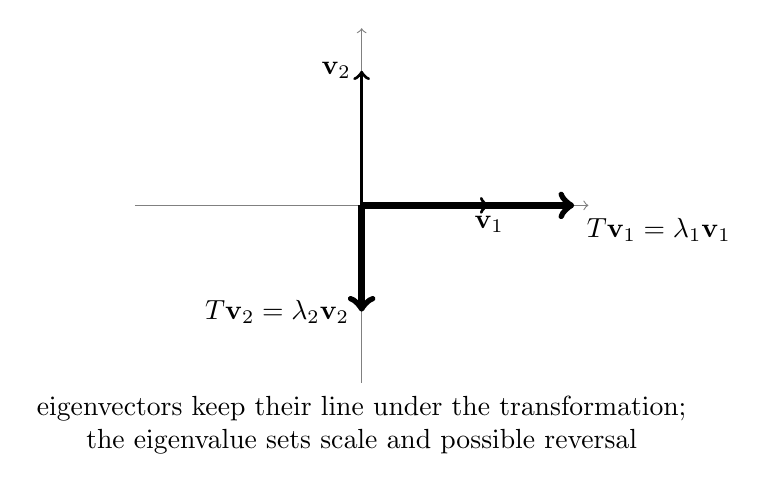
\begin{tikzpicture}[scale=0.9]
  \draw[->,gray] (-3.2,0)--(3.2,0); \draw[->,gray] (0,-2.5)--(0,2.5);
  \draw[->,very thick] (0,0)--(1.8,0) node[below] {$\mathbf v_1$};
  \draw[->,line width=2.4pt] (0,0)--(3.0,0) node[below right] {$T\mathbf v_1=\lambda_1\mathbf v_1$};
  \draw[->,very thick] (0,0)--(0,1.9) node[left] {$\mathbf v_2$};
  \draw[->,line width=2.4pt] (0,0)--(0,-1.5) node[left] {$T\mathbf v_2=\lambda_2\mathbf v_2$};
  \node[align=center] at (0,-3.1) {eigenvectors keep their line under the transformation;\\the eigenvalue sets scale and possible reversal};
\end{tikzpicture}
